\documentclass[tikz]{standalone}

\usepackage[T1]{fontenc}
\usepackage[english]{babel}

\usepackage{tikz}

\usepackage{pgfplots}


\begin{document}
    \pgfplotsset{every tick label/.append style={font=\tiny}}
	\begin{tikzpicture}
		\node[visible on=<1-2>] (dsm) at (0,0) {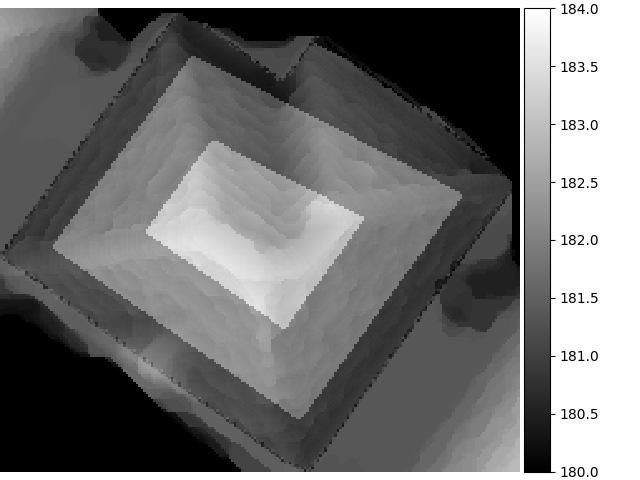
\includegraphics[width=3cm]{images/features/scatnet/dsm}};
        \path (dsm.south) node[anchor=north, text width=3cm, align=center, visible on=<1-2>] (dsm_legend) {\scriptsize \acrshort{acr::dsm}};

        \path (dsm.east) node[anchor=west, visible on=<2>] (minus) {\Large --};

		\path (minus.east) node[anchor=west, visible on=<2>] (model) {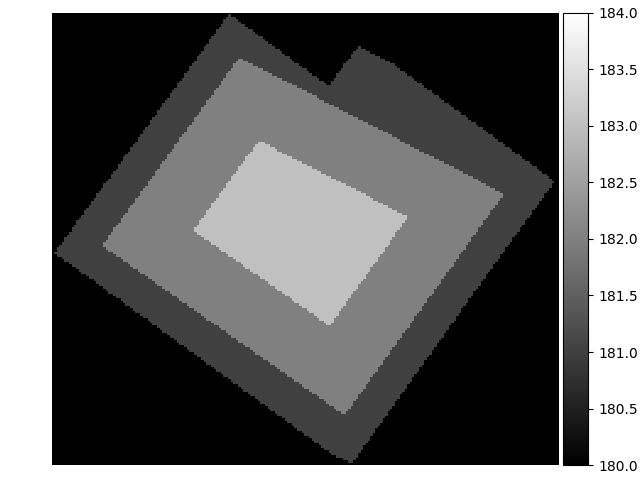
\includegraphics[width=3cm]{images/features/scatnet/height_map}};
        \path (model.south) node[anchor=north, text width=3cm, align=center, visible on=<2>] (model_legend) {\scriptsize Model height};

        \path (minus) node[visible on=<3>] (residual) {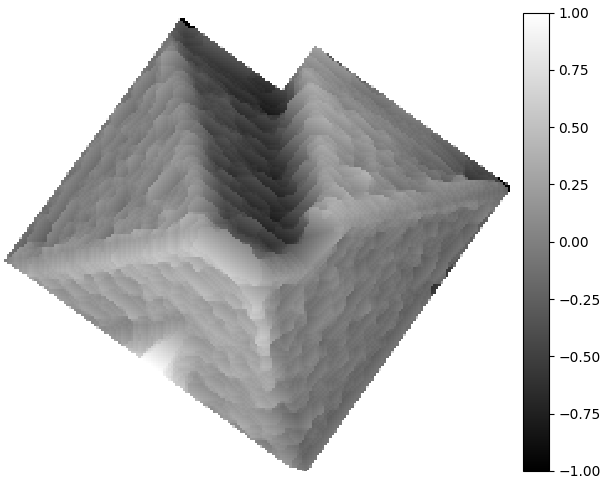
\includegraphics[width=3cm]{images/features/scatnet/residual_colbar}};
        \path (residual.south) node[anchor=north, text width=3cm, align=center, visible on=<3>] (residual_legend) {\scriptsize Residual};

        \path (residual.west) node[anchor=east, visible on=<3>] (equals) {\Large =};

        \path (dsm.west) node[anchor=west, visible on=<4->] (residual) {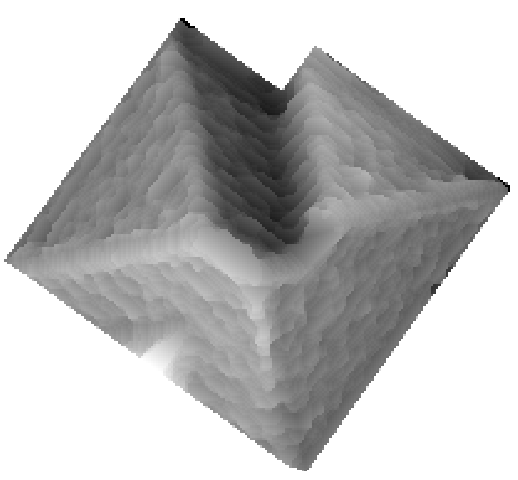
\includegraphics[width=1.5cm]{images/features/scatnet/residual}};
        \path (model.east) node[anchor=east, visible on=<4->] (hist) {
            \resizebox{1.5cm}{1cm}{
				\begin{tikzpicture}
					\begin{axis}[
                        area style,
                        ymin=0,
                        xmin=-14,
                        xmax=14,
                        visible on=<4->
                    ]
                        \addplot+[ybar interval,mark=no] plot coordinates {
                            (-15, 0) 
                            (-14, 0)
                            (-13, 876)
                            (-12, 366)
                            (-11, 593)
                            (-10, 675)
                            (-9, 2231)
                            (-8, 3623)
                            (-7, 546)
                            (-6, 159)
                            (-5, 182)
                            (-4, 70)
                            (-3, 54)
                            (-2, 123)
                            (-1, 3815)
                            (0, 4291)
                            (1, 211)
                            (2, 10)
                            (3, 0)
                            (4, 0)
                            (5, 0)
                            (6, 0)
                            (7, 0)
                            (8, 0)
                        };
                    \end{axis}
				\end{tikzpicture}
			}
        };

        \draw[->, very thick, visible on=<4->, black] (residual) -- (hist) node[midway, visible on=<4->, draw, rounded corners, black, fill=white] {Histogram};
	\end{tikzpicture}
\end{document}
